\documentclass[a4paper, 11pt]{article} % Font size (can be 10pt, 11pt or 12pt) and paper size (remove a4paper for US letter paper)

\usepackage[protrusion=true,expansion=true]{microtype} % Better typography
\usepackage{graphicx} % Required for including pictures
\usepackage{hyperref}
\usepackage{float}

 \usepackage{natbib}

\usepackage{mathpazo} % Use the Palatino font
\usepackage[T1]{fontenc} % Required for accented characters
\linespread{1.05} % Change line spacing here, Palatino benefits from a slight increase by default

\makeatletter
\renewcommand\@biblabel[1]{\textbf{#1.}} % Change the square brackets for each bibliography item from '[1]' to '1.'
\renewcommand{\@listI}{\itemsep=0pt} % Reduce the space between items in the itemize and enumerate environments and the bibliography

\renewcommand{\maketitle}{ % Customize the title - do not edit title and author name here, see the TITLE block below
\begin{flushright} % Right align
{\LARGE\@title} % Increase the font size of the title

\vspace{50pt} % Some vertical space between the title and author name

{\large\@author} % Author name
\\\@date % Date

\vspace{40pt} % Some vertical space between the author block and abstract
\end{flushright}
}

%----------------------------------------------------------------------------------------
%	TITLE
%----------------------------------------------------------------------------------------

\title{\textbf{PhyloGeoTool}\\ % Title
User Reference Manual} % Subtitle

\author{\textsc{Ewout Vanden Eynden, Pieter Libin, Kristof Theys, anderen, Guy Baele} % Author
\\{\textit{Rega Institute for Medical Research, KU Leuven}}} % Institution

\date{August 2016} % Date

%----------------------------------------------------------------------------------------

\begin{document}
\maketitle % Print the title section

\vspace{30pt} % Some vertical space between the abstract and first section

%------------------------------------------------
\tableofcontents
\newpage

This document provides additional information on how to use the PhyloGeoTool once it's installed (as described in the Installation Manual).
A deployed version of the PhyloGeoTool can be found at \url{http://regatools.med.kuleuven.be/phylogeotool/PhyloGeoTool}.

\section{Tool functionality}

\subsection{Required input files}

\begin{itemize}
\item How do we get started with a typical visual exploration in the PhyloGeoTool? 
\item What are the required input files a user needs to upload before the visual exploration can start? If this is covered in the installation manual, we should mention it here. If nothing more is needed after deployment, we should mention that as well.
\end{itemize}


\subsection{Basic functionality}




\begin{figure}[H]
\centering
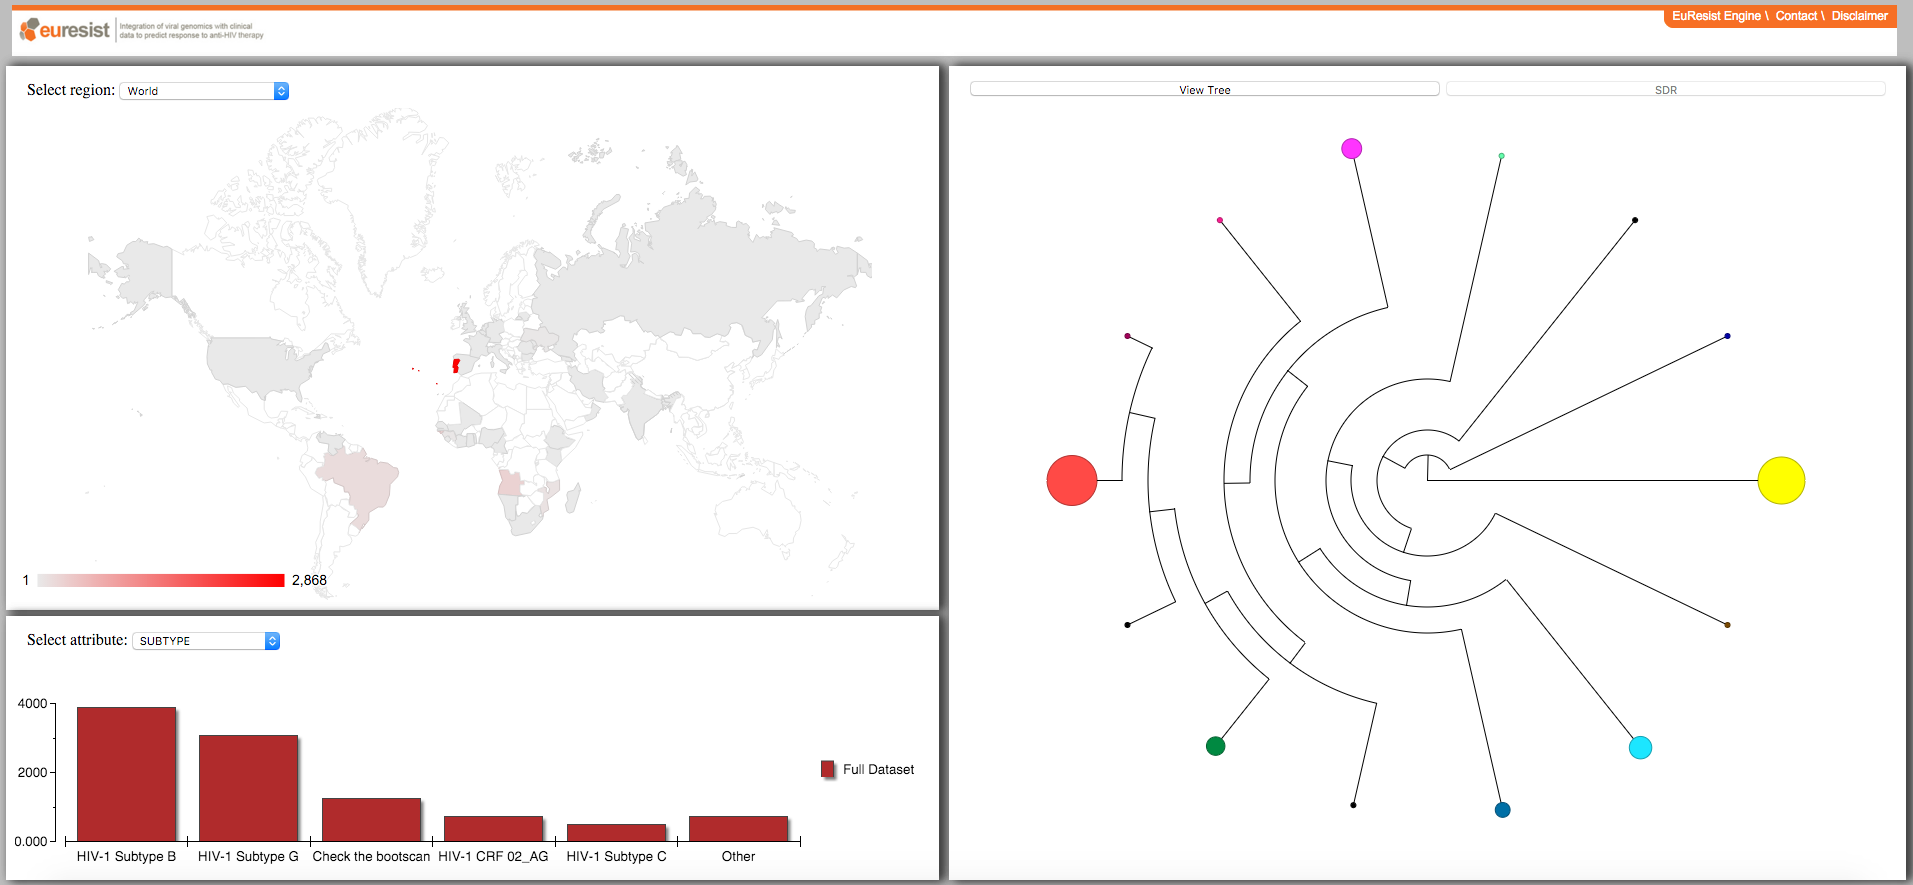
\includegraphics[width=400pt, height=400pt, keepaspectratio=true]{images/initial_view.PNG}
\caption{Initial view of the tool}
\label{fig:initial_view}
\end{figure}

The tool is divided into different area's
\begin{itemize}
  \item Top left shows a world map where each country is colored darker as more sequences are originating from here. It also contains a drop down box where you can select the region on which you want to zoom in (e.g. Europe, North-America, \ldots).
  \item Bottom left shows a bar chart which shows a certain attribute/characteristic from all sequences currently shown in the circular tree on the right. It also contains a drop down box where you can select the attribute/characteristic that you want to display in the bar chart. The attributes available for representation depend on the attributes given in the csv file.
  \item On the right, initially, the best clustering of the phylogenetic tree is shown. It also contains a button to visualise the tree in FigTree format.
\end{itemize}

\subsubsection{Hover over node in clustered tree}
\begin{figure}[H]
\centering
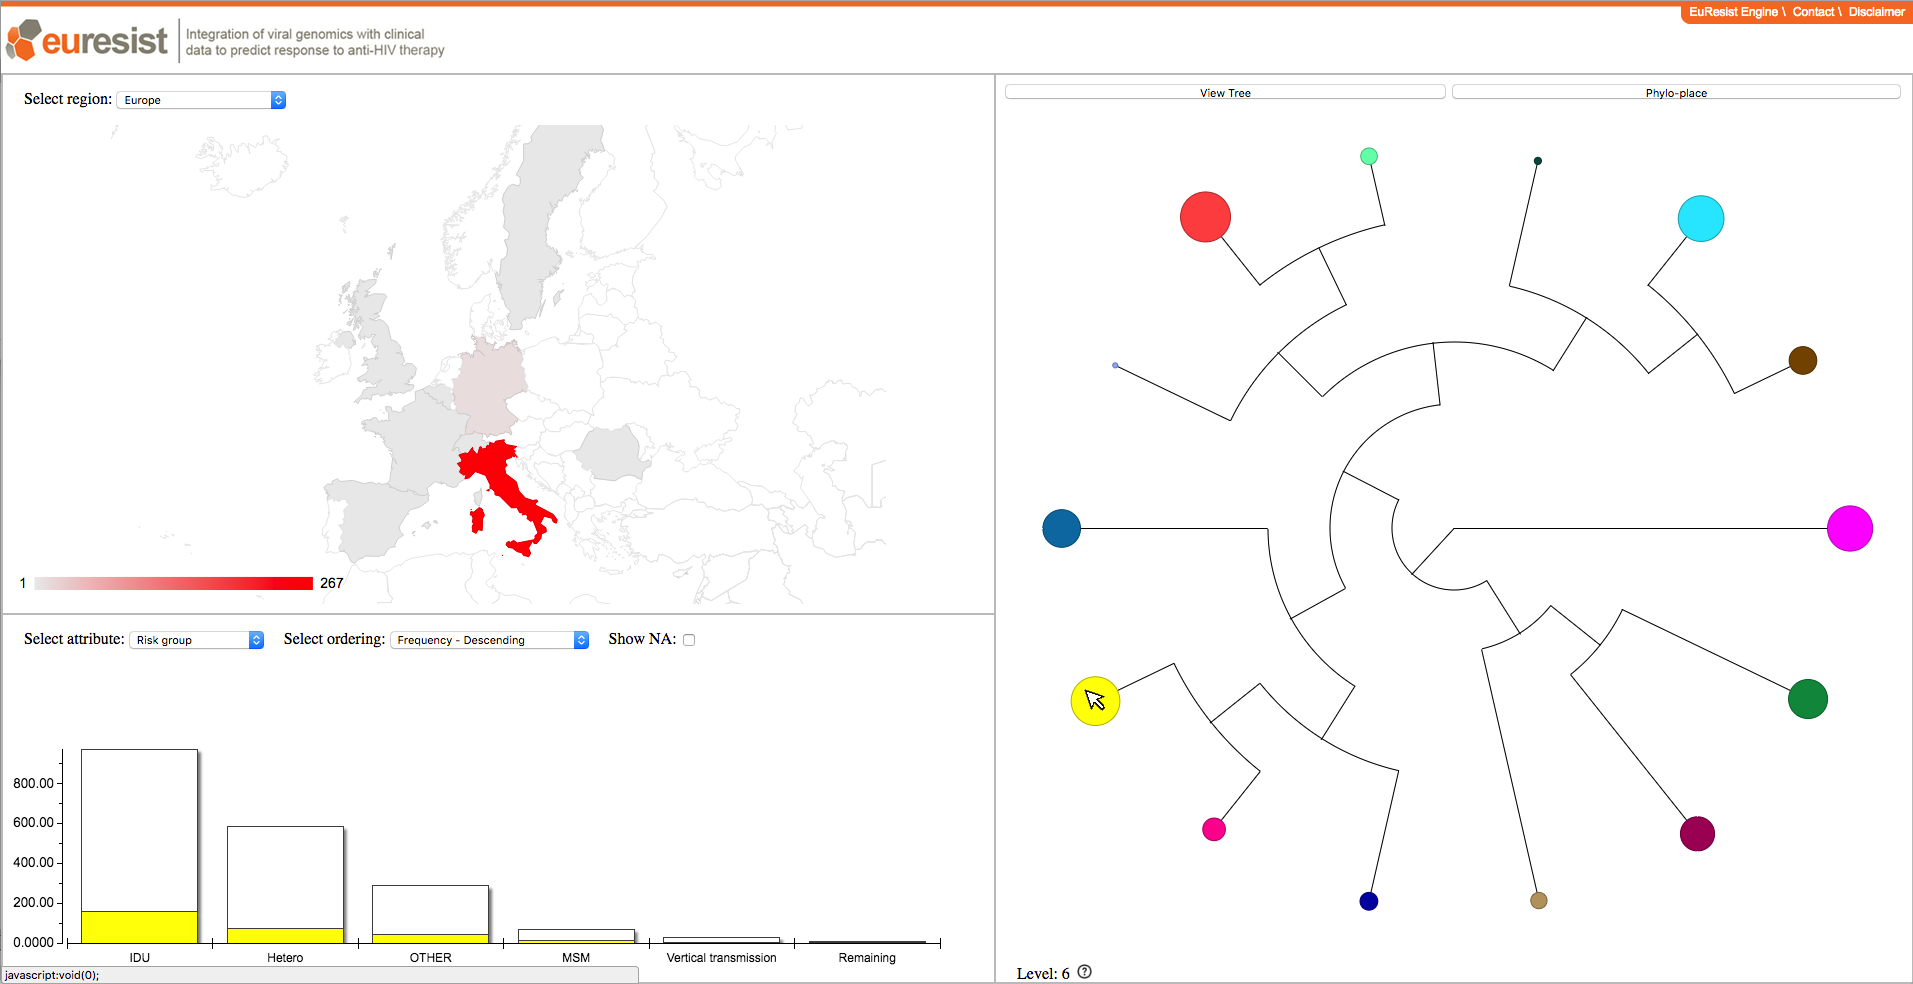
\includegraphics[width=400pt, height=400pt, keepaspectratio=true]{images/hover_node.PNG}
\caption{Hovering over a node in the tree}
\label{fig:hover_node}
\end{figure}

When you hover over a node in the phylogenetic tree, the bar chart on the bottom left and the map on the top left will be updated with data coming specifically from the node you hovered over.
\\
In the bar chart it'll be shown as an extra column that is added next to the already visible column.
\\
On the map it'll be shown as a new country colouring where each country is coloured based on only information coming from the hovered node.

\subsubsection{Change region}
\begin{figure}[H]
\centering
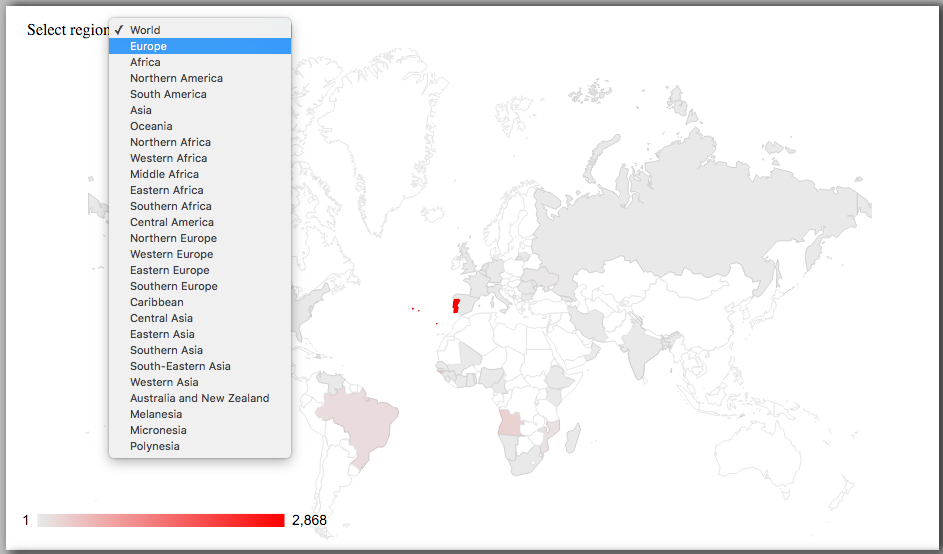
\includegraphics[width=400pt, height=400pt, keepaspectratio=true]{images/change_country.PNG}
\caption{Change the region in the drop down box}
\label{fig:change_region}
\end{figure}
When you change the region by selecting a new value in the drop down box on top of the map (see fig. \ref{fig:change_region}), the world map will update and now only show information originating from this specific region.

\subsubsection{Change attribute}
\begin{figure}[H]
\centering
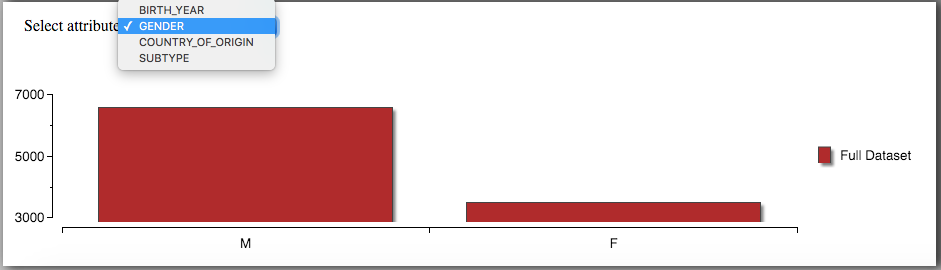
\includegraphics[width=400pt, height=400pt, keepaspectratio=true]{images/change_attr.PNG}
\caption{Change the attribute in the drop down box}
\label{fig:change_attr}
\end{figure}
When you change the attribute by selecting a new value in the drop down box on top of the bar chart (see fig. \ref{fig:change_attr}), the chart will update and now only show data for this specific newly selected attribute.

\subsubsection{View Tree}
\begin{figure}[H]
\centering
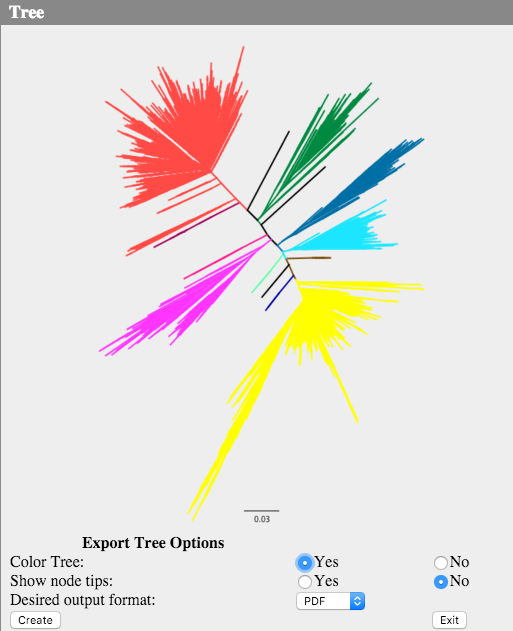
\includegraphics[width=400pt, height=400pt, keepaspectratio=true]{images/view_tree.PNG}
\caption{Tree visualization in FigTree}
\label{fig:view_tree}
\end{figure}
When the 'View Tree' button on top of the circular phylogenetic tree representation is clicked, a popup window will appear such as in fig. \ref{fig:view_tree} where the tree is shown as a radial tree such as it is represented in FigTree. The different clusters get different colours. The colours in the radial tree representation correspond to the colours in the circular tree representation.
\\
In addition to the visualisation of the tree, export options are available. The user can select if he/she wants the tree to be coloured, if the node tips should be shown and in which format the tree will be exported. 

\subsection{PPlacer}
Explanation of the PPlacer here. Not enough relevant data yet. Should be added here. \citep{Matsen2010}

Using PPLacer, additional sequences can be added to a previously reconstructed phylogenetic tree.
To do so, select PPlacer in the clustering window; there are two ways to add a new sequence to the tree:
\begin{itemize}
\item Paste the nucleotide sequence you'd like to add in the presented window.
\item Choose a Fasta file containing the nucleotide sequence using the file chooser.
\item Fasta files containing multiple sequences are allowed up to a total of MAX sequences, which will be placed sequentially into the phylogenetic tree.
\end{itemize}



\section{Example: exploring an HIV-1 data set}

In this section, we provide an example application of the PhyloGeoTool on HIV-1 using data available within the EuResist Integrated Data Base \citep{Zazzi2012}. 
This database contains virus genotypes, clinical responses and epidemiological markers of more than 66.000 patients from 12 different countries.

\bibliographystyle{natbib}%%%%natbib.sty
\bibliography{References}%%%refs.bib

\end{document}
